% !TEX encoding = UTF-8
% !TEX TS-program = pdflatex
% !TEX root = ../tesi.tex
% !TEX spellcheck = it-IT

%**************************************************************
\chapter{Introduzione}
\label{cap:introduzione}
%**************************************************************

%Introduzione al contesto applicativo.\\

%\noindent Esempio di utilizzo di un termine nel glossario \\
%\gls{api}. \\

%\noindent Esempio di citazione in linea \\
%\cite{site:agile-manifesto}. \\

%\noindent Esempio di citazione nel pie' di pagina \\
%citazione\footcite{womak:lean-thinking} \\

%**************************************************************
\section{L'azienda}

VIC è stata fondata da Alessio Bisutti che, dopo aver sviluppato una lunga esperienza
nel campo ispettivo, ha deciso di costituire una società in grado di offrire ai propri clienti un servizio professionale, chiaro ed affidabile, appoggiandosi alle nuove tecnologie.
Si occupa di controlli per grandi ordini, sia di materie prime che di semi-lavorati, di
cui individua e riporta eventuali danni, carenze nella spedizione e non conformità con
quanto ordinato.
VIC viene fondata a Venezia 7 anni fa come piccola società di ispezione locale. Fin dall'inizio, l'obiettivo principale di VIC è stato la riduzione del tempo tra ispezione e reporting al cliente. Ora l'obiettivo è raggiunto, perchè VIC sta fornendo ai suoi clienti tutti i risultati e le informazioni importanti in tempo reale, senza alcun ritardo, grazie agli investimenti fatti nel campo della tecnologia e delle applicazioni mobili.

%**************************************************************
\section{L'idea}

I più importanti obbiettivi del controllo qualità effettuato durante un ispezione sono il determinare la corretta forma, peso, quantità e dimensioni degli oggetti da esaminare.\\
Gli ispettori possono scattare fotografie, prendere appunti e sfruttare la loro esperienza per fornire stime accurate; si è manifestata però la necessità di affiancare queste ultime a dei dati quanto più possibile oggettivi e rapidi da ottenere.\\
Da qui nasce l'idea di fornire agli ispettori uno strumento informatico in grado di effettuare queste stime. Grazie alla ricostruzione computerizzata resa disponibile dai \emph{Tango device} sarà possibile non solo visualizzare su uno schermo il modello 3D del soggetto della ispezione, ma anche ottenere ulteriori dati utili quali:
\begin{itemize}
	\item Una stima del volume, e se necessario del peso, dell'oggetto.
	\item L'esito del confronto dell'oggetto con un modello ideale, per evidenziare eventuali danni o deformazioni.
\end{itemize}
Con il prototipo realizzato durante lo \emph{stage} sono rese disponibili solamente le funzionalità di ricostruzione dell'oggetto e calcolo (approssimato) del volume.\\
Le operazioni troppo computazionalmente intensive da effettuare su tablet, quali il filtraggio e \emph{meshing} dei punti acquisiti, sono state delegate ad un \emph{backend server} che effettui le elaborazioni necessarie ed invii i risultati al richiedente, mentre all'applicativo per tablet è stato affidato il compito di aquisire e visualizzare un oggetto sotto forma di 'Nuvola di Punti' e poterne esaminare la \emph{mesh} ottenuta.

%**************************************************************
\section{Cos'è Project Tango}

Project Tango è un \emph{tablet} sperimentale prodotto da \emph{Google} in grado di scandire tridimensionalmente l'ambiente circostante e di tracciare la propria posizione rispetto ad esso. Ciò è possibile attraverso il ricco hardware di cui è dotato (si veda la figura \ref{fig:tango_hardware}), tra cui:
\begin{itemize}
\item una fotocamera RBG-IR\\
\item una fotocamera \emph{Fisheye}\\
\item un sensore di profondità IR\\
\item accelerometro e giroscopio\\
\end{itemize}

\begin{figure}[!h] 
    \centering 
    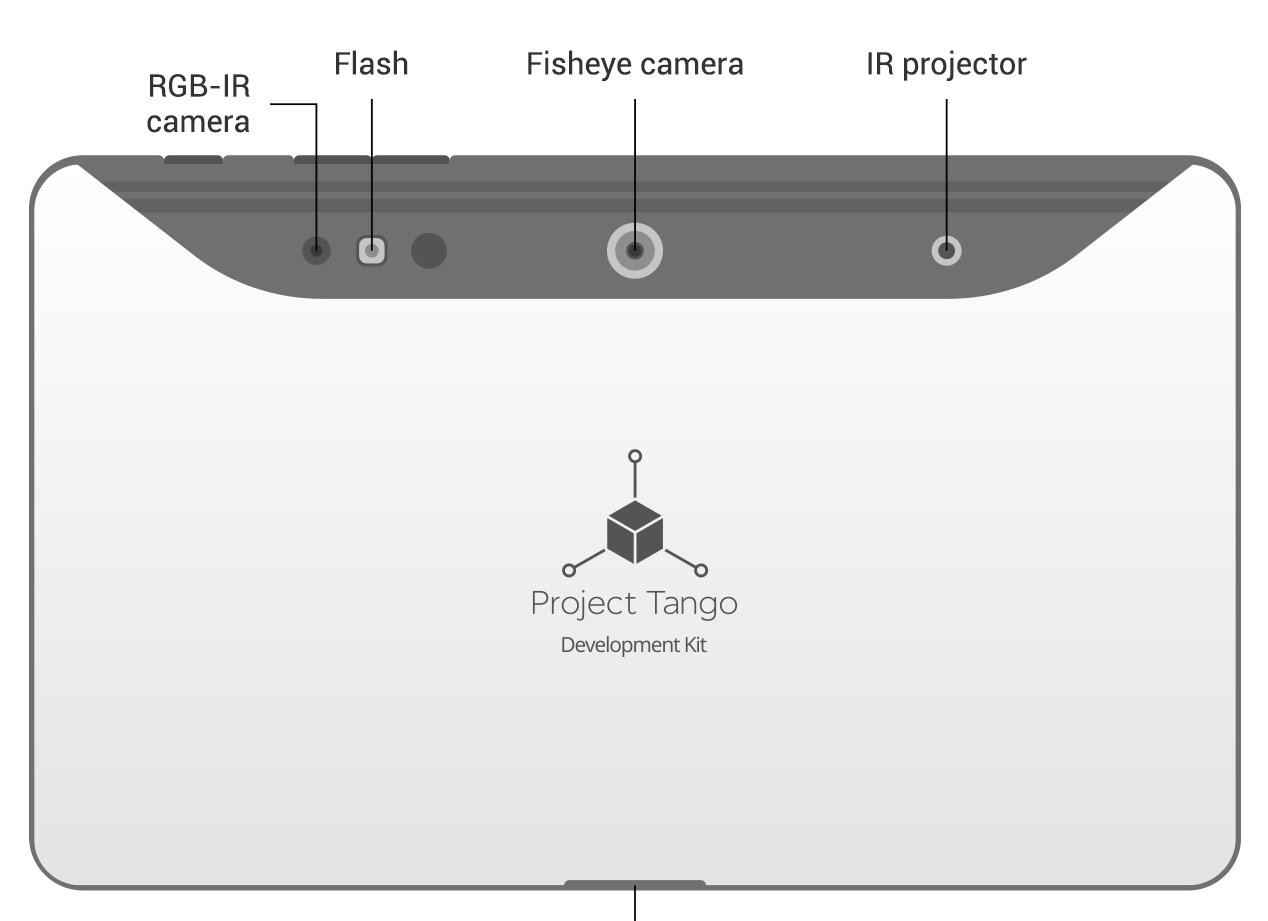
\includegraphics[width=0.9\columnwidth]{varie/tango-hardware.png} 
    \caption{L' \emph{hardware} di \emph{Project Tango}}
    \label{fig:tango_hardware}
\end{figure}

\noindent
Project Tango è quindi specificamente pensato per sviluppare applicazioni che necessitano di comprendere ed estrapolare informazioni dal mondo reale (ad es. realtà aumentata).
Le funzionalità del \emph{tablet} sono accessibili attraverso le \emph{Tango API}, le \emph{API} ufficiali per lo sviluppo di applicazioni \emph{Tango}.


%**************************************************************
\section{Il Prodotto - lato client}

L'applicazione su \emph{tablet} prodotta realizza, seppur non in maniera completa, le esigenze citate al punto precedente. \\
La sua realizzazione ha incontrato molte problematiche talvolta critiche e difficili da prevedere. Per questo durante lo sviluppo sono stati implementati più prototipi, al fine di esplorare le potenzialità e soprattutto i limiti del \emph{tablet} e delle \emph{Tango API}. \\
Lo scopo principale dell'applicazione lato \emph{tablet} è quello di rilevare una corretta 'Nuvola di Punti' dell'oggetto che si vuole esaminare.\\
Una 'Nuvola di Punti' è una descrizione matematica di un oggetto tridimensionale ottenuta tramite un insieme, il più possibile fitto, di punti che lo compongono, definiti dalle loro coordinate (\textbf{x},\textbf{y},\textbf{z}) rispetto ad un fissato sistema di riferimento. \\
Tale rappresentazione, riferita spesso d'ora in poi con il più elegante termine inglese \emph{Point Cloud}, è facilmente comprensibile all'utente se visualizzata come in figura \ref{fig:point_cloud_example}.
\begin{figure}[!h] 
    \centering 
    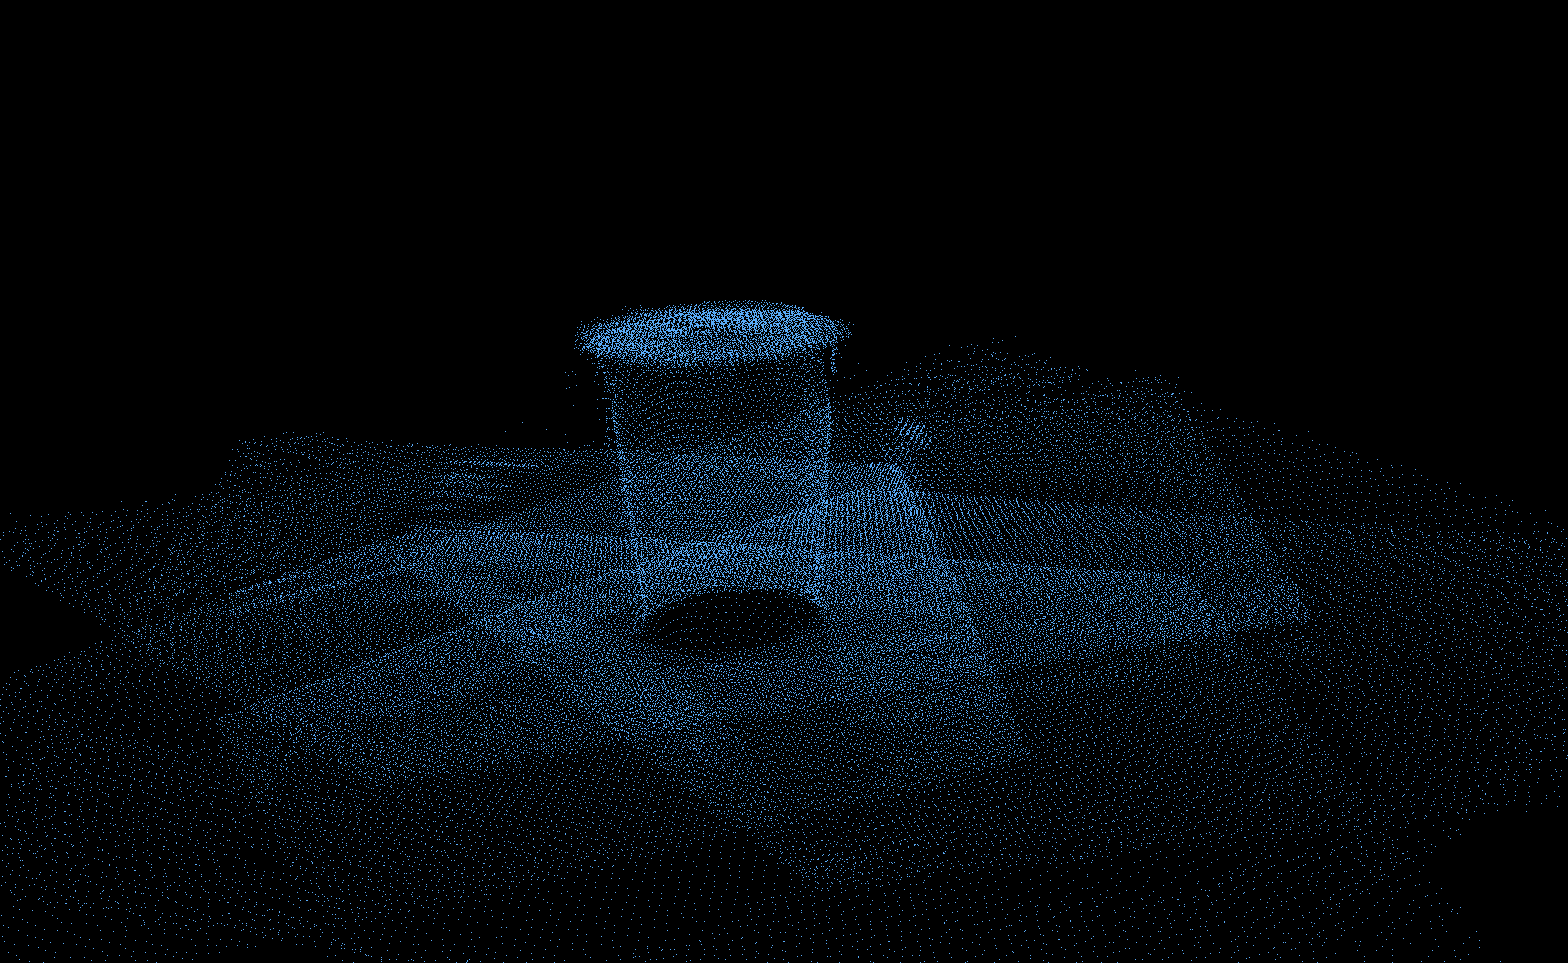
\includegraphics[width=1.0\columnwidth]{varie/point_cloud_example.png} 
    \caption{Esempio di \emph{Point Cloud}: un cestino cilindrico}
   \label{fig:point_cloud_example}
\end{figure}

\subsection{Primo prototipo: Cloude}
Il prototipo denominato \emph{Cloude} risponde all'esigenza di catturare più \emph{Point Cloud} da più angolazioni in modo da ricostruire l'oggetto scansionato sovrapponendo i dati acquisiti. \emph{Cloude} è il risultato di più prototipazioni precedenti effettuate dallo stagista che ha iniziato il progetto prima di me e con cui ho strettamente collaborato.\\
Il prototipo permette quindi di acquisire più \emph{Point Cloud} in successione, ognuno dei quali verrà adeguatamente ruotato e traslato rispetto allo spostamento del \emph{tablet}, in modo che la sovrapposizione degli stessi vada infine a ricostruire tutte le parti dell'oggetto esaminato.\\
Una sola acquisizione da una certa angolazione non può infatti comprendere un oggetto nella sua interezza, come dimostrato nelle figure //TODO è necessario ricostruire passo per passo un unico \emph{Point Cloud} rappresentante l'oggetto completo.
Sulla base dei risultati di \emph{Cloude} ho iniziato il mio lavoro sulla parte di elaborazione lato \emph{server} dei \emph{Point Cloud} acquisiti; questo è stato inoltre il punto di inizio per lo sviluppo dei prototipi successivi in collaborazione con l'altro stagista.

\subsection{Secondo prototipo: Samba}


\subsection{L'applicativo attuale: VIC-Tango}

%**************************************************************
\section{Il Prodotto - lato server}



%**************************************************************
\section{Organizzazione del testo}
Riguardo la stesura del testo, relativamente al documento sono state adottate le seguenti convenzioni tipografiche:
\begin{itemize}
	\item gli acronimi, le abbreviazioni e i termini ambigui o di uso non comune menzionati vengono definiti nel glossario, situato alla fine del presente documento;
	\item per la prima occorrenza dei termini riportati nel glossario viene utilizzata la seguente nomenclatura: \emph{parola}\glsfirstoccur;
	\item i termini in lingua straniera o facenti parti del gergo tecnico sono evidenziati con il carattere \emph{corsivo}.
\end{itemize}